\chapter{系统功能需求分析与系统架构设计}

\section{系统功能需求}
在一确定的CNN中,卷积的计算时间占据了至少85\%\cite{chen2017eyeriss},因此若想制作一款卷积神经网络加速器,那么急需解决的问题就是如何加速图像的卷积计算。
卷积计算虽然参数相比于CNN中全连接层少,但其计算量非常大,而且通常为简单的乘加操作,十分适合并行计算。

同时小型嵌入式设备对功耗十分敏感,而从外部DDR中取数据所需要的功耗是从片上SRAM中取数据的数百倍\cite{chen2016eyeriss},因此为了解决功耗问题,需要一种充分复用数据的卷积方法来减少对外部DDR的交互,最大化每个数据的利用率。
而且,为了方便与异构处理器集成,所开发的加速器要接口简单、易于控制。

因此,本文所设计的卷积神经网络加速器需要具备高算力、低功耗、接口易于控制的特性。

本文设计的卷积神经网络加速器生成器需要具备以下技术指标:
\begin{figure}[h]
    \begin{itemize}[topsep = 0 pt]
        \setlength{\topsep}{0pt}
        \setlength{\itemsep}{0pt}
        \setlength{\parsep}{0pt}
        \setlength{\parskip}{0pt}
        \setlength{\partopsep}{0pt}
        \item 支持8bit,16bit定点数计算
        \item 支持多通道、多卷积核、多图片的常规卷积操作
        \item 支持ReLu激活
        \item 支持自动化生成任意规模大小的计算阵列
        \item 一个计算单元一秒能够进行$10^8$次乘加操作
        \item 一个5×7的计算阵列的资源占用需要满足ZYNQ-CLG400 FPGA的资源限制
    \end{itemize}
\end{figure}

\section{系统架构设计}
    针对本章第一节的需求,本文通过调研当前硬件加速方案,参考文献\cite{chen2017eyeriss}、文献\cite{chen2016eyeriss}的思想和文献\cite{sun2018high}中的架构设计了一套针对CNN计算加速的方案。
    \begin{figure}[h]
        \centering
        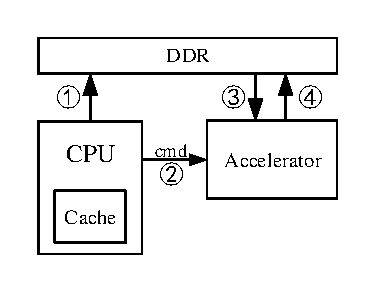
\includegraphics{../pdf/system.pdf}
        \caption{CNN加速系统架构示意图}
        \label{sys}
    \end{figure}
    工作时,CPU可以发挥自身强大的调度能力从外部存储器(硬盘,SD卡)读取数据,将数据放在约定好的DDR地址处如图\ref{sys},1号箭头所示。
    数据准备好之后CPU发出开始计算命令,如图\ref{sys},2号箭头所示。
    加速器接受到指令之后,从DDR约定好的位置拉取数据,如\ref{sys},3号箭头,进行计算,结果写回DDR指定地址,如图\ref{sys},4号箭头所示。
    至此一轮计算完成,CPU可以通过读取DDR获得计算结果。

% \section{开发环境}
%     \subsection{HLS}
%     HLS(High Level Synthesis)也既高层次综合技术,是Xilinx公司大力推广的一项FPGA开发技术。该技术使用C/C++作为开发语言,可以充分利用该语言中提供的数据结构进行FPGA开发。
%     最终可以生成Verilog或VHDL语言。

%     通过HLS使得软件工程师可以不用了解FPGA和Verilog,也可以使用FPGA进行硬件加速,大幅减少FPGA开发难度和开发周期。该技术已应用在SDAccel、SDSoC等软件中,目前在偏算法的视频图像处理领域有着广泛的应用。

%     但简单易用的东西背后都会带来不必要的性能浪费。与传统HDL开发相比,HLS无法对电路进行精细化操作,因此虽然HLS能够大大缩短开发周期,但从能性能方面传统HDL开发更具有优势。
%     \subsection{OpenCL}
%     HLS可以进行算法的快速实现,但是并不适合大规模系统开发。OpenCL的出现给人们带来使用高层次综合进行大规模系统开发的希望。
%     OpenCL(Open Computing Language)即开放运算语言,是第一个面向异构系统通用目的并行编程的开放式、免费标准,也是一个统一的编程环境,广泛使用于CPU,GPU,DSP,FPGA等并行处理器的开发。
%     其提供了一系统采用C/C++封装的API,编写的程序可以在支持OpenCL的设备上运行。
%     与HLS相似,OpenCL也使开发人员脱离底层电路,允许在系统层面进行开发。由于OpenCL是跨平台的,因此可以很容易的将原来CPU或GPU的代码做些许改动就能在支持OpenCL的FPGA上运行。
% \section{敏捷型开发}
%     敏捷型开发思想源于软件工程,其宗旨是以用户需求进化为核心,采用迭代、循序渐进的方法进行软件开发,在此过程中软件一直处于可工作状态。软件之所以可以采用敏捷型开发是因为其反馈环足够短,同时软件开发工具成熟易用。
%     而目前数字芯片公司大多对敏捷性开发很陌生,事实上芯片开发周期长已经是阻碍数字芯片设计快速发展的重要瓶颈。传统数字芯片公司大多采用Verilog的同时,还需使用一些非标准的Python/Perl等脚本语言进行代码编写自动化任务,
%     而然这种方式可移植性差,同时调试比较困难。
%     \begin{figure}[h]
%         \centering
%         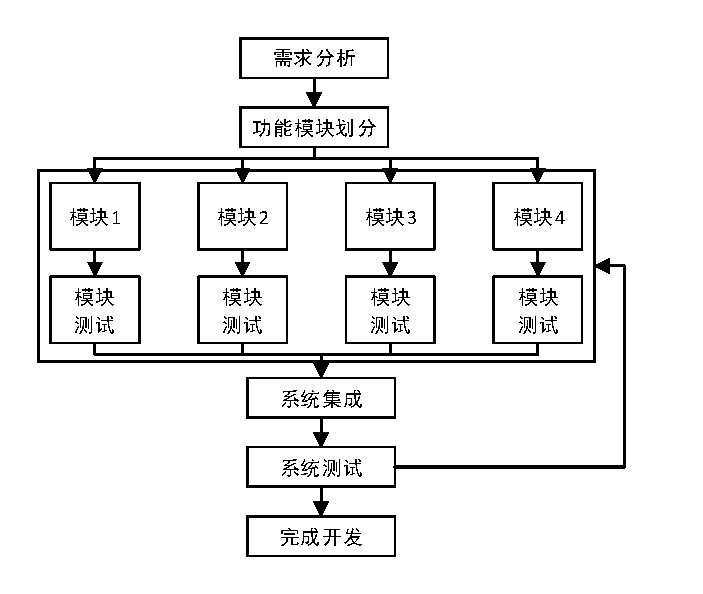
\includegraphics{../pdf/tradition.pdf}\\
%         \caption{传统开发流程图}
%         \label{tra}
%     \end{figure}
%     \begin{figure}[h]
%         \centering
%         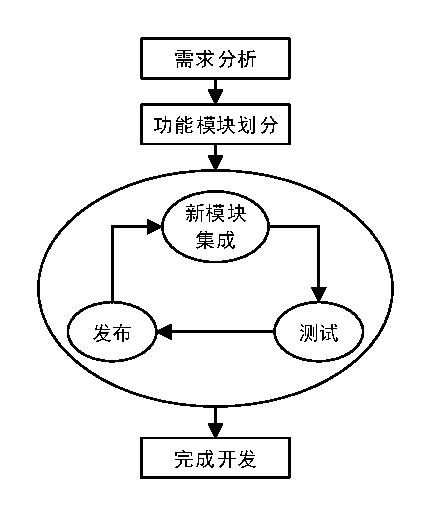
\includegraphics{../pdf/agile.pdf}\\
%         \caption{敏捷型开发流程图}
%         \label{agi}
%     \end{figure}
%     传统的开发流程可以参考图\ref{tra},可以发现开发流程呈线性,当前阶段完成后只需关注后续阶段,但用户只有等到整个过程末期才能见到开发效果,增加了开发风险,同时灵活性较低。
%     敏捷型开发流程可以参考图\ref{agi},其主要开发过程呈现环状,当发布第一版之后便可见到项目雏形,同时具有高适应性可以随着开发深入遇见的问题随时调整方向。

\section{基于行静止思想的卷积计算方法}
如本章第二节所述,计划采用CPU+FPGA实现卷积神经网络的计算加速。
\begin{figure}[h]
    \centering
    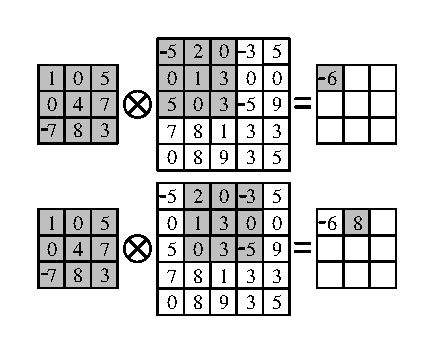
\includegraphics{../pdf/tra_conv.pdf}\\
    \caption{图像卷积计算流程}
    \label{tra_conv}
\end{figure}
传统图像卷积计算流程如图\ref{tra_conv} 所示,卷积核先与图像第一行第一列开始的同等大小矩阵进行点乘运算,计算结果进行累加得到结果的第一个值,然后卷积核在图像上向右进行滑动,再次进行点乘累加运算即可得到第二个值。
通过滑动卷积核,即可得到整张图片的卷积结果。
可以看出,若不加干预,传统卷积计算方式并没有充分缓冲数据,因为每次计算一次卷积都需要重新获取新的图片数据,这将大大更加与DDR的交互工作,一方面增加了传输数据的时间,另一方面提高了功耗。

\begin{figure}[h]
    \centering
    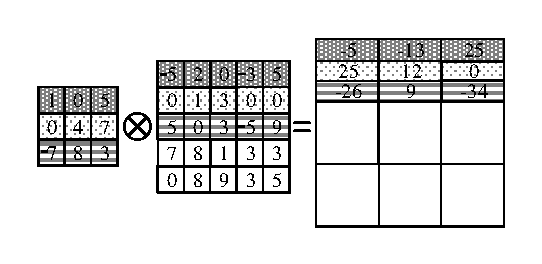
\includegraphics{../pdf/row_conv.pdf}\\
    \caption{行静止卷积计算流程}
    \label{row_conv}
\end{figure}
基于行静止思想的卷积的计算模式如图\ref{row_conv} 所示,其与普通的卷积计算模式不同,首先卷积核的第一行和图像的第一行进行一维卷积操作(图中阴影背景所标出的部分),计算结果进行缓存。
之后卷积核第二行和图像的第二行进行一维卷积操作(图中斑点背景标出部分),卷积结果和上一次按位置进行累加。
最后卷积核和图像的第三行进行一维卷积计算,得到的结果再次进行按位置累加操作,即可得到最终结果的第一行。
然后卷积核的第一、二、三行分别于图像的二、三、四行进行一维卷积操作,即可得到最终结果的第二行。
通过迭代此过程即可得到完整的卷积结果。

这种计算模式虽然不能减少计算次数,但是十分适合硬件去进行数据缓存以减少与DDR进行交互的能量消耗,因为每次加速器都会从DDR中一次性加载一行的filter数据和img数据,然后进行一维卷积,其所需的变换和数据移动可以完全在寄存器之间完成,大大减少了能量消耗。
同时这种,行静止计算方式,非常适合做并行加速,因为一行与一行之间的一维卷积完全独立,最后计算的结果按位置进行累加即可得到最终正确结果。



\section{本章小结}
本章首先对比传统计算架构介绍了选择异构计算的优势,其次介绍了目前主流的一些快速开发FPGA的技术,再其次引出采用Chisel3进行硬件敏捷型开发的优势及其流程,最后引出了本文所设计的加速器的核心思想。

% \subsection{二级节标题}

% \subsubsection{三级节标题}

% \paragraph{四级节标题}

% \subparagraph{五级节标题}

% \section{脚注}

% Lorem ipsum dolor sit amet, consectetur adipiscing elit, sed do eiusmod tempor
% incididunt ut labore et dolore magna aliqua. Ut enim ad minim veniam, quis
% nostrud exercitation ullamco laboris nisi ut aliquip ex ea commodo consequat.
% Duis aute irure dolor in reprehenderit in voluptate velit esse cillum dolore eu
% fugiat nulla pariatur. Excepteur sint occaecat cupidatat non proident, sunt in
% culpa qui officia deserunt mollit anim id est laborum.
% \footnote{This is a long long long long long long long long long long long long
% long long long long long long long long long long footnote.}
